\documentclass{standalone}
\usepackage[dvipsnames,svgnames,x11names]{xcolor}
\usepackage{tikz}
\usepackage{../thesismath}
\begin{document}
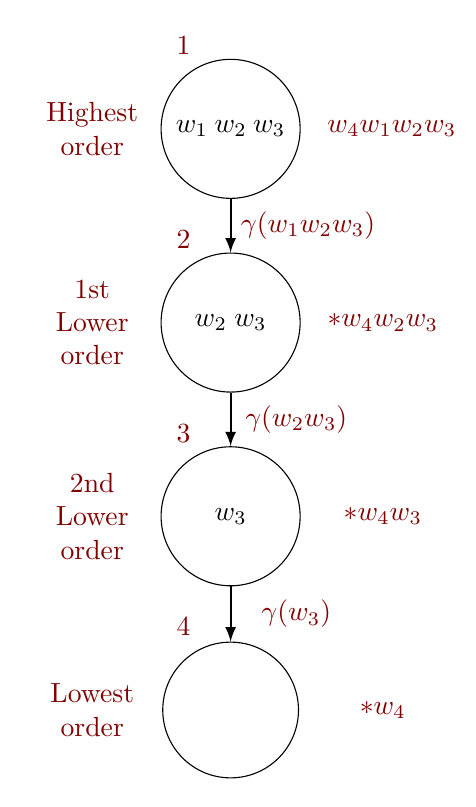
\begin{tikzpicture}
  \tikzset{
    state/.style  = {draw, circle, align = center, text centered, text width = 4.2em},
    invis/.style  = {text width = 4.2em},
    order/.style  = {align = center, text centered, text width = 4em, text = Maroon},
    number/.style = {xshift = -1.7em, text = Maroon},
  }

  \begin{scope}[node distance = 7em]
    \node [state] (highest)                    {$w_1 \: w_2 \: w_3$};
    \node [state] (lower1)  [below of=highest] {$w_2 \: w_3$};
    \node [state] (lower2)  [below of=lower1]  {$w_3$};
    \node [state] (lowest)  [below of=lower2]  {$\EmptyNGram$};
  \end{scope}

  \begin{scope}[node distance = 5.5em]
    \node [order] [right of=highest] {$\ProbMKN {w_4}{w_1 w_2 w_3}$};
    \node [order] [right of=lower1]  {$\ProbMKN*{w_4}{w_2 w_3}$};
    \node [order] [right of=lower2]  {$\ProbMKN*{w_4}{w_3}$};
    \node [order] [right of=lowest]  {$\ProbMKN*{w_4}$};
  \end{scope}

  \begin{scope}[node distance = 5em]
    \node [order] [left of=highest] {Highest order};
    \node [order] [left of=lower1]  {1st Lower order};
    \node [order] [left of=lower2]  {2nd Lower order};
    \node [order] [left of=lowest]  {Lowest order};
  \end{scope}

  \begin{scope}[node distance = 3em]
    \node [number] [above of=highest] {1};
    \node [number] [above of=lower1]  {2};
    \node [number] [above of=lower2]  {3};
    \node [number] [above of=lowest]  {4};
  \end{scope}

  \path[->, >=latex, thick]
    (highest) edge node [right, order] {$\textstyle{\gamma(w_1 w_2 w_3)}$} (lower1)
    (lower1)  edge node [right, order] {$\textstyle{\gamma(w_2 w_3)}$}     (lower2)
    (lower2)  edge node [right, order] {$\textstyle{\gamma(w_3)}$}         (lowest);
\end{tikzpicture}
\end{document}
